% \documentclass[letterpaper, 10 pt, conference]{ieeeconf}  % Comment this line out if you need a4paper

\documentclass[a4paper, 10pt, conference]{ieeeconf}    % Use this line for a4 paper

\IEEEoverridecommandlockouts                              % This command is only needed if 
                                                          % you want to use the \thanks command

\overrideIEEEmargins                                      % Needed to meet printer requirements.

%In case you encounter the following error:
%Error 1010 The PDF file may be corrupt (unable to open PDF file) OR
%Error 1000 An error occurred while parsing a contents stream. Unable to analyze the PDF file.
%This is a known problem with pdfLaTeX conversion filter. The file cannot be opened with acrobat reader
%Please use one of the alternatives below to circumvent this error by uncommenting one or the other
%\pdfobjcompresslevel=0
%\pdfminorversion=4

% See the \addtolength command later in the file to balance the column lengths
% on the last page of the document

% The following packages can be found on http:\\www.ctan.org
%\usepackage{graphics} % for pdf, bitmapped graphics files
%\usepackage{epsfig} % for postscript graphics files
%\usepackage{mathptmx} % assumes new font selection scheme installed
%\usepackage{times} % assumes new font selection scheme installed
%\usepackage{amsmath} % assumes amsmath package installed
%\usepackage{amssymb}  % assumes amsmath package installed

\usepackage{graphicx}
\usepackage{amsmath}
\usepackage[utf8x]{inputenc}
\usepackage[dvipsnames]{xcolor}
% \usepackage[demo]{graphicx}
% \usepackage{caption}
\usepackage{subcaption}
\usepackage{float}

\begin{document}

\title{\LARGE \bf
Descrição da equipe TauraBots para LARC/CBR 2019 na Categoria IEEE Very Small Size Soccer
}





\author{Junior C. Jesus$^{1}$, Maurício M. Godoy$^{1}$, Jair A. Bottega$^{1}$,\\ Bruno S. Castro$^{1}$, Renan M. Chiesa$^{1}$, Gabriel N. Niederauer$^{1}$ e Álisson H. Kolling$^{1}$% <-this % stops a space
% \thanks{*This work was not supported by any organization}% <-this % stops a space
\thanks{$^{1}$Todos estudantes são do grupo TauraBots de competição, da Universidade Federal de Santa Maria
        {\tt\small taurabots.ufsm@gmail.com}}%
}
% de Tecnologia em Automação em Robótica Aplicada <- O "TauraBots" grupo de competição não é um acrônimo

\maketitle
\thispagestyle{empty}
\pagestyle{empty}


%%%%%%%%%%%%%%%%%%%%%%%%%%%%%%%%%%%%%%%%%%%%%%%%%%%%%%%%%%%%%%%%%%%%%%%%%%%%%%%%

\begin{abstract}

Este documento descreve o desenvolvimento feito pela equipe TauraBots da Universidade de Santa Maria para participação da LARC/CBR 2019 na categoria IEEE \textit{Very Small Size Soccer}.
É dado detalhe da construção da parte mecânica, elétrica e comunicação dos robôs que serão utilizados na competição. Para a parte de estratégia é definido o sistema de visão que será capaz de apresentar os dados necessário para que uma rede de aprendizado por reforço profundo consiga dar ações para que os robôs criados consigam jogar futebol contra outros times tentando maximizar a sua vitória.

\end{abstract}

\keywords
Visão Computacional, Futebol, Robótica, Aprendizado por Reforço Profundo.
\endkeywords


%%%%%%%%%%%%%%%%%%%%%%%%%%%%%%%%%%%%%%%%%%%%%%%%%%%%%%%%%%%%%%%%%%%%%%%%%%%%%%%% 
\section{INTRODUÇÃO}

A categoria IEEE \textit{Very Small Size Soccer} (VSSS), é uma competição robótica de futebol entre duas equipes de três robôs de dimensões de até 7,5x7,5x7,5cm. 
A competição ocorre dentro de um campo fabricado com uma chapa plana e rígida com dimensões de 150x130cm, na cor preta. Esse campo é delimitado por paredes com quatro cantos em forma de triângulos isósceles sólidos de dimensões 7x7cm, de cor branca e parte superior de cor preta. 
O controle dos robôs é feito por um computador, denominado de técnico. Toda estratégia de jogo é controlada de forma autônoma, ou seja, sem intervenção humana. 
Para realizar esse controle é utilizada uma câmera de vídeo fixada a uma altura não inferior a 2 metros de altura do campo. 
A câmera tem a função de fornecer informações visuais de posicionamento tanto dos robôs da equipe quanto dos adversários dentro do campo.
O reconhecimento por visão computacional dos robôs é feito através de \textit{tags}, posicionadas na parte superior do robô. Essas \textit{tags} identificam o robô através do uso de cores para determinar o time ao qual pertencem, sendo possível utilizar as cores amarela ou azul. O uso de um número maior de \textit{tags} é permitido e optativo, contanto que não sejam iguais às cores utilizadas pela equipe adversária, e servem para identificar cada robô separadamente. A Figura \ref{fig:esquematico} exemplifica a organização do campo utilizado na prova.
% O parágrafo abaixo foi reescrito no parágrafo acima. De nada :)
%O reconhecimento por visão computacional dos robôs é feito através de \textit{tags} posicionadas na parte superior do robô, sendo no mínimo a tag de identificação da equipe do robô podendo ser ela na cor amarela ou azul, as demais tags são optativas da equipe para identificar cada robô separadamente, podendo ter qualquer cor exceto a cor da tag de identificação da equipe adversária. Uma ideia do campo da prova é mostrado na Figura \ref{fig:esquematico}.

\begin{figure}[htbp]
\centerline{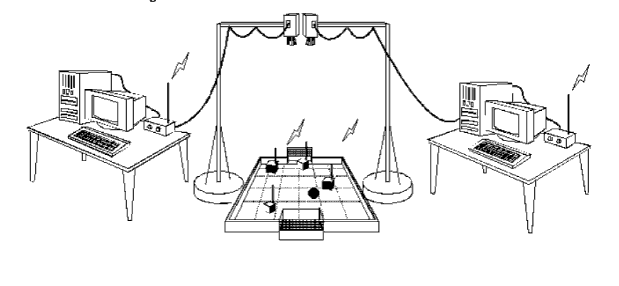
\includegraphics[width=\columnwidth]{capitulos/imagens/Esquematico-de-uma-partida-do-IEEE-VSSS.png}}
\caption{Ambiente da prova}
\label{fig:esquematico}
\end{figure}

Todas as jogadas e estratégias são definidas de forma autônoma pelo técnico, que através dos dados recebidos, envia por meio de uma rádio transmissor qual jogada ou estratégia utilizar durante a jogada para cada robô separadamente.

A equipe TauraBots, fundada no ano de 2015, pelo Professor Dr. Rodrigo da Silva Guerra com o intuito de desenvolver robótica dentro do Centro de Tecnologia (CT) da Universidade Federal de Santa Maria (UFSM), concorrendo principalmente em categorias de robôs humanoides, passando a se envolver recentemente com outras áreas da robótica como carros autônomos e robótica móvel. Participará pela primeira vez este ano na categoria VSSS na presente competição, que vem sendo disputada no Brasil desde o ano de 2003. A equipe que tem como principais conquistas primeiro lugar na RoboCup 2018 na competição de arquearia robotica e terceiro lugar na mesma categoria na AutCup no Irã, terceiro lugar em nos LARC's de 2015 e 2016 na competição Robocup Humanoid League e um terceiro lugar na RoboCar Race no Brasil.

O artigo será dividido em cinco seções. Na seção \ref{construction} será explicado o processo de construção dos robôs e os componentes utilizados, assim como a justificativa de sua escolha.
Na seção \ref{vision} será explicado o sistema de visão utilizado pela equipe. Na seção \ref{strategy} será explicado o sistema de estratégia utilizado na competição. 
Por fim, na seção \ref{conclusion} será apresentada a conclusão do presente artigo.

\section{CONSTRUÇÃO DOS ROBÔS}\label{construction}
%% Bruno S. Castro Autor ==================================

Esta secção será destinada à descrição técnica das principais características do robô, referente às suas composições mecânicas e eletrônicas. Além disso, apresentaremos a justificativa das escolhas e seus respectivos benefícios.

\subsection{Estrutura Externa}
%% Bruno S. Castro Autor ==================================

Levando em consideração a facilidade de chegar a estrutura desejada, o custo de produção, trabalho manual envolvido e tempo necessário para construção, decidimos utilizar, após vários testes, impressão 3D com filamento ABS, preenchimento XX\%, altura da camada de XX mm, bico de XX mm e as temperaturas de mesa XX ºC e do bico XX ºC. 

O resultado desta decisão pode ser observado na Figura \ref{fig:visometrica} e superou expectativas, pois obtivemos uma estrutura bem leve (aproximadamente XX gramas), porém suficientemente resistente e modular, com a possibilidade de trabalhar separadamente nos compartimentos mecânico ou eletrônico devido a sua divisão interna, a qual aparenta o robô como um H.

\begin{figure}[htbp]
\centerline{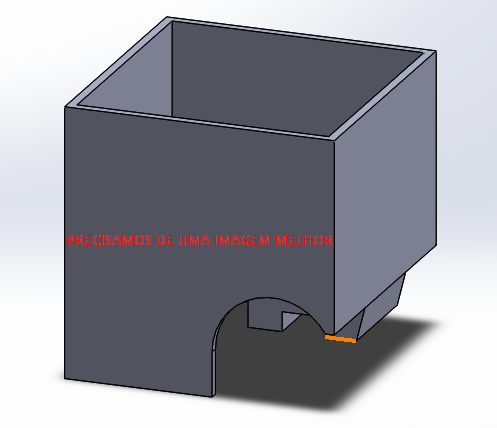
\includegraphics[width=\columnwidth]{capitulos/imagens/robo_visometrica.png}}
\caption{Projeto 3D do robô em vista isométrica}
\label{fig:visometrica}
\end{figure}

Quando o robô precisar de manutenção, podemos ir diretamente ao compartimento mecânico onde temos acesso aos sistemas de movimentação do servo-robô, ou seja, acesso direto aos motores, rodas e conexões entre eles, tal como a fiação elétrica do robô e a bateria de fácil remoção.
Já quando houver a necessidade de acesso ao compartimento eletrônico, teremos contato direto com o sistema de controle responsável pela Rede de Comunicação (disponível na subseção \ref{subsec:rede_com}) do robô. 

\subsection{Sistema de Movimentação}\label{subsec:sist_mov}
%% Bruno S. Castro Autor ==================================

Abaixo descrevemos a composição do nosso Sistema de Movimentação, como pode ser visto na Figura \ref{fig:sist_moviment}, o qual vai ser controlado pela Rede de Comunicação (disponível na subseção \ref{subsec:rede_com}).

\subsubsection{Rodas}
%% Bruno S. Castro Autor ==================================
Quanto ao sistema físico de movimentação do robô, estamos utilizando uma roda composta por um pneu feito com borracha de silicone ultra-resistente de dureza 15 Shore-A acoplado a um cubo de roda feito em Alumínio 6351-T6 especificamente para este pneu. Estes podem ser analisados na Figura \ref{fig:roda}.

\subsubsection{Motores}
%% Bruno S. Castro Autor ==================================
E para completar nosso sistema de movimentação, usamos dois Micro Motores de 6V com caixa de redução para 600 RPM, os quais tem seu eixo fixado as rodas citadas anteriormente. O motor pode ser analisado na Figura \ref{fig:motor}.

\begin{figure}[htbp]
\centering
\begin{subfigure}{0.25\textwidth}
  \centering
  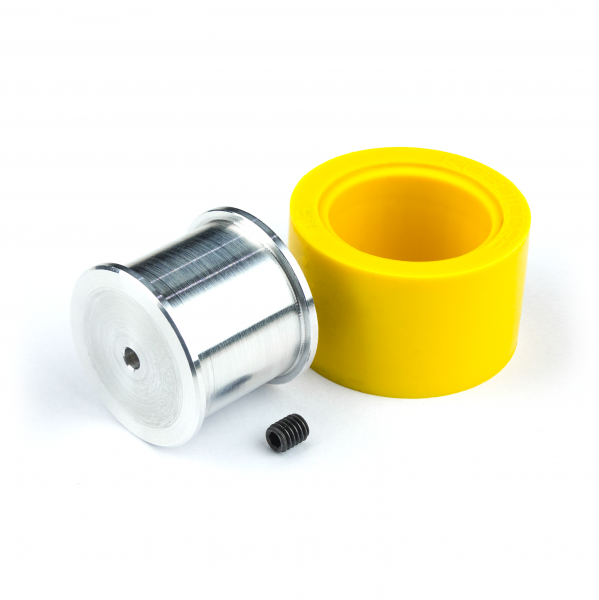
\includegraphics[width=.9\linewidth]{capitulos/imagens/roda_sep.png}
  \caption{Roda utilizada}
  \label{fig:roda}
\end{subfigure}%
\begin{subfigure}{0.25\textwidth}
  \centering
  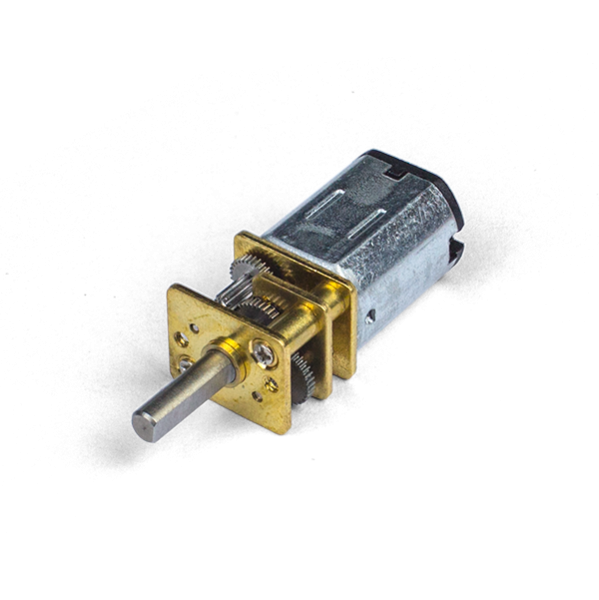
\includegraphics[width=.9\linewidth]{capitulos/imagens/motor.png}
  \caption{Micro Motor utilizado}
  \label{fig:motor}
\end{subfigure}
\caption{Componentes do Sistema de Movimentação}
\label{fig:sist_moviment}
\end{figure}



\subsection{Rede de Comunicação}\label{subsec:rede_com}

\subsubsection{Módulos Receptores}\label{subsec:recept_models}
%% Renan M. Chiesa ==================================

Neste quesito a equipe buscou um sistema de comunicação com uma largura de banda considerável, baixa latência e difícil interferência.
A escolha lógica se afrontou para os módulos de comunicação Xbee\textsuperscript{\textregistered} S2C, os quais se destacam nesses aspectos, porém não possuem um preço adequado para um projeto que não utiliza o envio de dados complexos. 
Desta maneira, buscando não alcançar o limite de projeto orçado, optamos por módulos de comunicação 2.4GHz genéricos mostrados na Figura \ref{fig:modulo_comunication}, estes não chegaram ao desempenho dos módulos Xbee, porém mostraram-se satisfatórios na ocasião. Este modulo possui taxas de transmissão e recepção entre 250kbps e 2Mbps com alcance de até 100 metros, podendo utilizar até 125 canais contendo seis endereços cada, possibilitando assim a conexão com até outras 6 unidades.

\begin{figure}[htbp]
\centerline{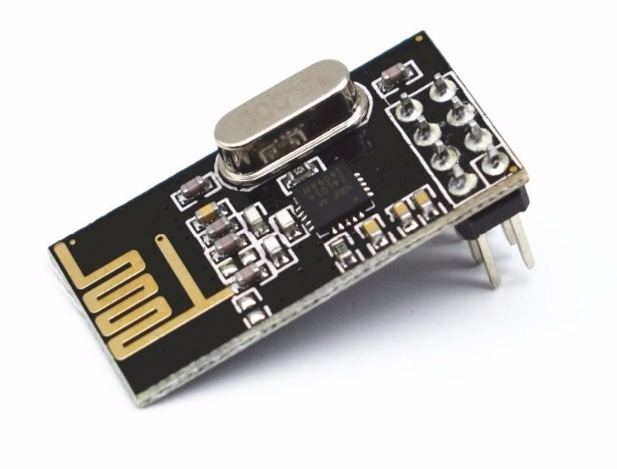
\includegraphics[width=\columnwidth]{capitulos/imagens/modulo_comunication.png}}
\caption{Módulo  NRF24L01}
\label{fig:modulo_comunication}
\end{figure}


\subsubsection{Base de Transmissão}
%% Renan M. Chiesa ==================================

Com o objetivo de estabelecer comunicação entre o sistema de processamento(computador) e cada robô, tivemos a necessidade de construir uma base de envio de dados remotos. Esta base é equipada com uma placa de desenvolvimento Arduino Mega e um módulo de comunicação 2.4 GHz idêntico aos inseridos nos robôs. Está placa foi programada para receber os dados do sistema de processamento por meio do protocolo serial USB, convertendo-os para a estrutura de dados a ser enviada. A comunicação é realizada na faixa de frequência de 2.4GHz(Wi-Fi), está configurada de modo a definir a base como mestre, e cada um dos receptores em modo servo, com estes três recebendo comandos remotos.

As mensagens a serem enviadas possuem formato pré-estabelecido pelo modelo do módulo. Serão enviados na mensagem, dados respectivos ao endereço do receptor do robô com que se deseja a comunicação e os dados necessários ao controle do robô. O envio ocorre várias vezes por segundo possibilitando assim um controle preciso. 


\subsection{Microcontrolador}
%% Alisson Autor ==================================

O microcontrolador escolhido pela equipe para controlar os robôs foi o ATmega328P embarcado na placa Arduino Nano. A preferência por este placa foi em decorrência de suas dimensões diminutas que são de 1,8 cm por 4,8 cm, mostrado na Figura \ref{fig:nano}. Possui todas funções básicas encontradas em placas Arduino porém apresentando algumas configurações diferenciadas, como a alimentação sendo realizada por uma entrada mini-USB e um menor número de portas de entrada e saída. As portas de entrada e saída encontradas nele são suficientes para a operação do robô. 

\begin{figure}[htbp]
\centerline{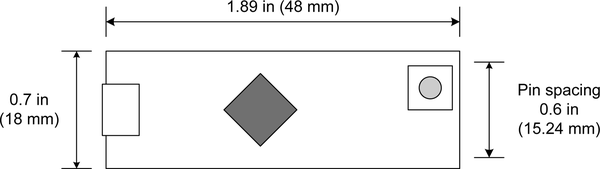
\includegraphics[width=\columnwidth]{capitulos/imagens/arduino_nano.png}}
\caption{Dimensões do Arduino Nano}
\label{fig:nano}
\end{figure}

\section{SISTEMA DE VISÃO}\label{vision}

O propósito da visão computacional é coletar dados do jogo em tempo real que tem como fim descrever o ambiente, e, posteriormente, transmití-los da forma mais compacta possível para o algoritmo responsável pela estratégia.
O processo para a extração dos dados do ambiente é descrito a seguir.
Primeiramente, uma câmera é fixada perpendicularmente ao campo, a aproximadamente 2 metros de altura, faz uma série de captura de imagens individuais, ou \textit{frames}, e os envia para o computador.
Para cada \textit{frame} recebido, utiliza-se um algoritmo para o processamento da imagem com base na biblioteca OpenCV \cite{bradski2008learning}.
Aplicam-se filtros na imagem para obter somente as partes importantes: a bola, as \textit{tags} de cores dos robôs da equipe, e as \textit{tags} da cor que identifica robôs da outra equipe.

Após serem detectadas as etiquetas de cores e a bola, um algoritmo é utilizado para calcular os dados necessários a ser usado como os estados para rede Deep-RL da estratégia, explicada na seção
\ref{strategy}.
Essa rede tem objetivo definir a tomada de decisão dos agentes após receber informações sobre o estado atual do jogo.
Alguns exemplos de dados enviados para a rede são: posição da bola, posição de robôs da equipe e adversários, orientação dos robôs em relação à bola, distância entre bola e gol, distância entre os robôs e a bola, dentre outros. 

O sistema de \textit{tags} de cores a ser utilizado para a detecção dos robôs no campo se dará pelo uso de 2 círculos de 4,5 centímetros de diâmetro cada, posicionados na diagonal.
Uma das etiquetas, localizada mais próxima à parte de trás do robô, possui a cor azul ou amarela, que serve para identificação do time.
A outra etiqueta possui uma cor distinta para cada robô, o que possibilita a diferenciação entre os robôs da equipe.
Através dos círculos, é possível extrair posição e orientação do robô em relação a bola.
A posição de um robô, por exemplo, é dada pelo ponto médio do vetor que liga o centro dos dois círculos.
O sistema de \textit{tags} pode ser visto na Figura $T A L$.

Algumas estratégias são utilizadas para reduzir o custo computacional. Por exemplo, após ter a posição de um robô em determinado \textit{frame}, o próximo processamento de detecção ocorrerá apenas em uma pequena parte da imagem, ao invés de percorrê-la por inteiro, deixando o processo mais otimizado.

\section{ESTRATÉGIA DE JOGO E TÉCNICAS DE CONTROLE}\label{strategy}

Para que os robôs sejam capazes de jogar, é necessário que haja estratégias de jogo, onde seja otimizada a chance de vitória dado o comportamento dos robôs. 
As decisões vão ser feitas através da analise dos dados coletados pela visão computacional, sendo assim definidas como estados da rede. 
A ação tomadas pelos robôs será feita através dos estados em que o ambiente atual do jogo vai estar. 
Esse controle pode ser feito através das técnicas de aprendizado por reforço exploradas em \cite{stone2005reinforcement} e \cite{riedmiller2009reinforcement}. 
%% Mas como os estados e ações no futebol são considerados de alta dimensão 

\subsection{Aprendizado por Reforço Profundo}

O objetivo do aprendizado por reforço profundo (Deep-RL) é controlar um agente em um ambiente na tentativa de maximizar a função de recompensa, mostrado na Figura \ref{fig:rl}.
O algoritmo da rede-Q profunda (DQN) \cite{mnih2013playing} foi capaz de ter um desempenho de nível humano em muitos dos jogos eletrônicos no Atari estimando as ações de um agente.
Contudo, enquanto a DQN pode resolver problemas em um espaço de observação complexo, ele só pode lidar com ações discretas. É possível notar que muitas tarefas, no controle de robótica, tem espaço de ações continuas.
Então a DQN não pode ser aplicada em domínios contínuos e é necessário usar um outro algoritmo capaz de lidar com esse tipo de problema.

\begin{figure}[htbp]
\centerline{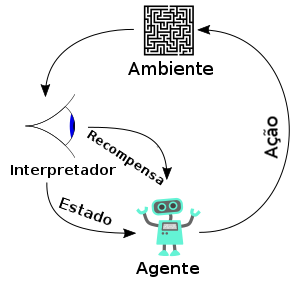
\includegraphics[width=\columnwidth]{capitulos/imagens/reinforcement_learning.png}}
\caption{Ideia principal do funcionamento do agente no Aprendizado por Reforço.}
\label{fig:rl}
\end{figure}

\subsubsection{Soft Actor-Critic (SAC)}

É um algoritmo de Deep-RL baseada na estrutura de entropia máxima para o aprendizado profundo \cite{haarnoja2017reinforcement}.
Nesta estrutura, o rede ator visa maximizar a recompensa esperada enquanto também maximizando a entropia.
Isto é, suceder em uma tarefa enquanto agindo tão aleatória como possível.
Este método é capaz de desempenhar varias atividades em aplicações de domínios contínuos \cite{haarnoja2018soft}.

\subsection{Função de Recompensa para Ataque e Defesa}

Para que a rede Deep-RL seja treinada é necessária uma função de recompensa que permita os agentes fazerem as ações que se é deseja.
Logo, é preciso formular um função de recompensa de ataque e defesa para que assim os agentes consigam jogar futebol.

As principais recompensas definidas para o jogo de futebol são as seguintes:
\begin{multline}
r (s_t, a_t) = r^{gol}_t + p^{gol}_t + c_1(d_{t-1}(b,g) - d_{t}(b,g))\\  + c_2(d_{t-1}(a,b) - d_{t}(a,b))
\end{multline}

Se a rede responsável pelas ações do agente fizer um gol uma recompensa $r^{gol}$ é dada e caso o time leve um gol uma recompensa negativa $p^{gol}$ é dada. Ambas condições representam a maiores recompensas que a rede pode receber por uma ação. 
Caso contrário, a recompensa é baseado na diferença da distância do intervalo de tempo atual com o tempo anterior $(d_{t-1}-d_t)$. Para que o agente se aproxime da bola é usado a distância do agente ao bola $d(a,b)$. Já para que a bola se aproxime do gol adversário é usado a distância da bola ao gol adversário $d(b,g)$.
%% Falta um pouquinho aqui



\section{CONCLUSÃO}\label{conclusion}

O VELHO BORA ESCREVD A COJNCLUASAO

Os resultados até então obtidos na modelagem e construção do robô, processamento de imagem e estratégia de jogo estão satisfatórios e em constante evolução.


Os resultados da aplicação dos métodos e técnicas apresentadas aqui estão sendo aprimorados mês após mês. O projeto do hardware vem sendo desenvolvido durante 4 anos e sofreu muitas mudanças de lá pra cá.
As novas técnicas empregadas no sistema de visão computacional mostraram ótimos resultados visto que a quantidade de frames processados aumentou consideravelmente devido a técnica de janelamento e o novo sistema de tags diminuiu a complexidade do algoritmo. Isso além de proporcionar um processamento maior auxilia no controle do robô, de acordo com as instruções enviadas pela estratégia.
O sistema de estratégia está passando por melhorias e ao mesmo tempo o método antigo está sendo aprimorado. 
A utilização de navegação por Univector Field e algoritmos
genéticos será utilizada para criação de modos de funcionamento dos robôs.
Neste sentido, visou-se mostrar aqui as principais partes e
divisões do projeto Very Small Size Soccer Team do Núcleo
de Robótica Pequi Mecânico do Instituto de Informática.
Como o projeto ainda está em andamento pequenas mudanças podem acontecer

\addtolength{\textheight}{-12cm}   % This command serves to balance the column lengths
                                  % on the last page of the document manually. It shortens
                                  % the textheight of the last page by a suitable amount.
                                  % This command does not take effect until the next page
                                  % so it should come on the page before the last. Make
                                  % sure that you do not shorten the textheight too much.

%%%%%%%%%%%%%%%%%%%%%%%%%%%%%%%%%%%%%%%%%%%%%%%%%%%%%%%%%%%%%%%%%%%%%%%%%%%%%%%%



%%%%%%%%%%%%%%%%%%%%%%%%%%%%%%%%%%%%%%%%%%%%%%%%%%%%%%%%%%%%%%%%%%%%%%%%%%%%%%%%



%%%%%%%%%%%%%%%%%%%%%%%%%%%%%%%%%%%%%%%%%%%%%%%%%%%%%%%%%%%%%%%%%%%%%%%%%%%%%%%%

%% se não quiser, só comentar essa parte
\section*{AGRADECIMENTOS}

Agradeço a nossas vós!!!



%%%%%%%%%%%%%%%%%%%%%%%%%%%%%%%%%%%%%%%%%%%%%%%%%%%%%%%%%%%%%%%%%%%%%%%%%%%%%%%%

\bibliographystyle{IEEEtran}
\bibliography{IEEEabrv,bibliography}



\end{document}
